% % CHAPITRE 1 : SYNTHESE BIBLIO
%
%Réflexions
%
%NE PAS OUBLIER DE CALER UN MAXIMUM D'ORDRE DE GRANDEUR ! 
%	(émissions CO2, CH4, stocks flux, surface des tourbières, végétation ...)
%
%Bien différencier l'intro générale qui doit être lisible par un béotien, de l'intro au travail de la thèse qui doit être un état de l'art précis et documenté sur les travaux antérieurs (synthèse biblio)
%
%Ou caler la partie de biblio sur l'expérimentation ... (peut être dans la synthèse biblio, paragraphe "approche mise en oeuvre"
%INTRODUCTION GENERALE (à mettre dans le chapitre Intro)
%
%- Qu'est ce qu'une tourbière ? (Éventuellememt comment se forme-t-elle ?)
%	*Définition
%	*Formation/Évolution (stockage du C, battement de la nappe ?)
%	*Classification
%- Les tourbières et les hommes 
%	*Usages d'hier et d'aujourd'hui (Combustible, horticulture, matériau de construction)
%	*Les thématiques scientifiques (pourquoi les avoir étudier et les étudier en gros)
%	*Le contexte dans lequel va s'inscrire le travail qui suit
%
%SYNTHESE BIBLIOGRAPHIQUE
%
%- Quelles sont les grandes thématiques de recherche liées aux tourbières ?
%	*Exploitation
%	*Archives
%	*Émissions de GES
%- Plus précisément quelles sont les grands axes de recherche sur ces écosystèmes et liés aux émissions de GES.
%	*Processus de création de GES (CO2 et CH4) (Facteurs contrôlant généralement invoqués)
%	*Processus de migration des GES dans le profil
%	*Processus de stockage/capture
%- Approches mise en oeuvre
%	*Modélisation (empirique et mécaniste)
%	*Expérimentation (différentes techniques pour mesurer les émissions de GES, différentes techniques de chambre...)
%	*Variabilité spatio-temporelle (notion d'échelle)
%	
%	DOIS-JE TRAITER
%	La classification des tourbières ?
%	Hummock and Hollow ? Dire qu'on n'est pas dans ce niveau de détail ?
%	
%
%HISTORIQUE (études concernant les tourbières)
%
%1968-1969  Boelter : propriétés physique des tourbes
%1977 Boelter : hydrologie, caractéristique des sols organiques, chimie des écoulements
%1978 Ingram : Classification
%1981 Parkinson : Déjà l'amélioration d'une méthode pour la mesure des émissions de la respiration du sol
%1984 Clymo : Les limites à la croissance des tourbières
%1986 Chason : Conductivités hydraulique et propriétés physiques
%1989 Moore : Influence du niveau de la nappe sur les émissions de CO2 et de CH4
%//1990 Raich : Comparaison de 2 méthodes de chambre statique pour mesurer les flux de CO2
%1991 Gorham : Rôle des tourbières dans le cycle du carbon et réponse au changement climatique
%//1992 Raich : Flux de CO2 dans la respiration du sol et relation vis à vis du climat et de la végétation
%1992 Roulet : Flux de méthane (fen) et changement climatique
%1993 Bubier : Émission de méthane dans les zones humides
%1993 Bubier : Microtopographie et flux de méthane dans tourbières boréales.
%1993 Abbès : Sorption de l'ammonium ? (ammonia) par la tourbe et fractionnement de l'azote
%1994 Lloyd : Dépendance de la respiration du sol à la température
%1994 Bubier : Perspective écologique sur les émissions de méthane dans les zones humide de l'hémisphère nord
%//1994 Nay : Biais des méthodes de chambre pour la mesure des flux de CO2
%1995 Kirschbaum : Dépendance à la température de la décomposition de la MO (effet sur stock de C et changement Clim)
%1995 Bubier : Prédiction des émissions de méthane à partir de la distribution des bryophytes (tourbière hémisphère nord)
%1995 Bubier : Contrôles "écologique" sur les émissions de méthane dans les tourbières de l'hémisphère nord
%1995 Bubier : Relation entre la végétation avec les émissions de méthane et les gradients hydrochimique
%//1995 Bekku : Mesure de la respiration du sol avec une méthode de chambre fermée (IRGA)

% PLAN (2015-03-03)
%I. Définitions
%1 Tourbières/Tourbe (surface, type, localisation, biodiversité, services écologiques...)
%2 Classification
%3 Historique
%	a Utilisation
%	b Études scientifiques
%	
%Transition : Réaction aux changements globaux (comment fonctionnent-elles ?)
%
%II. Fonctionnement
%1 Stock
%2 Flux
%	a Entrants (Photosynthèse)
%	b Sortants (Méthanogénèse, Respiration)
%3 Facteurs Contrôlant
%	a Hydrologie (WTL,HR)
%	b Propriétés physiques (T, densités, conductivités thermiques...)
%	c Végétation (Bryophytes/Vasculaires)
%	d Météo

% GO TO intro générale ?
%Depuis quand sont-elles étudiées ?
%D'abord étudiées pour leurs propriétés physiques afin de connaitre leur qualité en tant que combustible.
%Elle sont maintenant majoritairement étudiée à travers le prisme des changements globaux.
%Ainsi les études concernent les flux de GES, ...

\chapter{Synth\`{e}se Bibliographique}

\minitoc

\newpage

\index{tourbières|(}
Dans ce chapitre, nous commenceront par donner une vue de ce que sont les tourbières : Que sont-elles ? Depuis quand sont-elles étudiées ? Pourquoi les a-t-on étudiés ?
Nous continuerons en entrant plus en détails sur leur fonctionnement vis à vis des flux de carbone.
Enfin nous verrons quels sont les facteurs contrôlant majeurs de ces flux.

\section{Les tourbières et le cycle du carbone}

\subsection{Zones humides et tourbières : définitions et terminologies}
Les tourbières font partie d'un ensemble d'écosystèmes plus large que l'on appelle les zones humides\index{zone humide}.
Ces zones humides ne sont ni des écosystèmes terrestres au sens strict, ni des écosystèmes aquatiques.
Elles sont à la frontière entre les deux et sont caractérisées par un niveau de nappe élevé, proche de la surface du sol, voire au dessus.
L'omniprésence de l'eau joue fortement sur l'aération du milieu et contraint, de façon plus ou moins importante, l'accès à l'oxygène.
De ces particularités, niveau de nappe élevé et accès à l'oxygène difficile, résulte le développement, dans ces écosystèmes, d'une végétation spécifique qui s'est adaptée aux milieux fortement humides ou inondés.
Les zones humides regroupent des écosystèmes très variés parmi lesquels les marais, les mangroves, les plaines d'inondations et les tourbières qui sont le siège d'une biodiversité spécifique.

Les tourbières représentent 50 à \SI{70}{\percent} des zones humides \cite{joosten2002}.
Elles sont généralement définies par rapport à la tourbe, qu'il convient donc de définir au préalable.
La tourbe est un sol organique (histosol) formé suite à l'accumulation de litières végétales partiellement décomposées dans un milieux saturé en eau.
Ce processus de formation est appelé la tourbification\index{tourbification}.
Les propriétés physiques de la tourbe dépendent du type de végétation, mais également de sa profondeur dans le profil (pédogenèse, diagenèse).

La définitions des tourbières est variable selon les régions (\plop, exple).
%Cela ne facilite pas leur recensement et leur cartographie.
Deux définitions sont régulièrement utilisées.
La première définie comme tourbières les écosystèmes possédant au moins \SI{30}{\cm} de tourbe (parfois 40).
Cette définition correspond au \textit{peatland} anglo-saxon.
La seconde définition considère comme tourbières les écosystèmes dans lesquels un processus de tourbification est actif.
Cette définition correspond au \textit{mire} anglo-saxon et peut être traduite en français par le terme de tourbière active.
Les deux concepts se chevauchent mais ne sont pas complètement similaire : une tourbière drainée peut avoir plus de \SI{30}{cm} de tourbe et ne plus être active.
À l'inverse il peut exister des zones ou l'épaisseur de tourbe est inférieure à \SI{30}{cm} malgré un processus de tourbification actif.

Ces variations de définitions ajoutées aux limites floues qui peuvent exister entre certain écosystèmes tourbeux et non-tourbeux rendent la cartographie de ces écosystèmes délicate.
Les estimations généralement citées évaluent la surface occupée par les tourbières à environ \SI{4000000}{\square\kilo\meter} \cite{lappalainen1996}.\index{tourbières!surface} 
Cette surface correspond à \SI{3}{\percent} de l'ensemble des terres émergées du globe.
Plus de \SI{85}{\percent} d'entre elles sont situés dans l'hémisphère nord, majoritairement dans les zones boréales et sub-boréales \cite{society2008}.

\begin{figure}
\centering
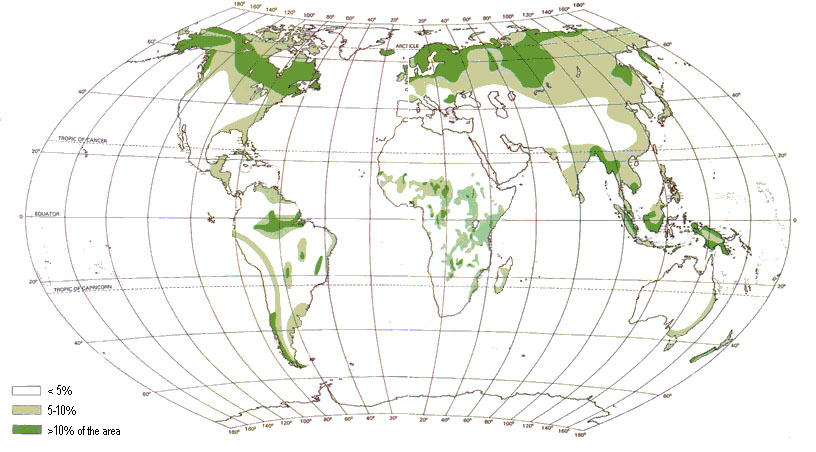
\includegraphics[width=\textwidth]{chap1/peatlandGlobalDistribution}
\caption{Global distribution of peatlands}
\label{fig:peatlandGlobalDistribution}\index{tourbières!distribution} 
\end{figure}

Différentes classifications sont utilisées pour classer ces écosystèmes.
De nombreux critères existent pour classer les tourbières selon leur mode de formation, leur source d'eau, leur physico-chimie.
La terminologie utilisée concernant ces écosystèmes n'a pas toujours été cohérente, de nombreux termes ont été utilisés parfois en contradiction les uns avec les autres \cite{joosten2002}.
Il existe différents types de tourbières, notamment on distingue des tourbières tempérées/boréales des tourbières tropicales dont le fonctionnement diffère.
Dans la suite de ce document seule les tourbières tempérées/boréales seront décrites et étudiées.

\subsection{Biodiversité dans les tourbières}
%\subsection{Les tourbières, des écosystèmes particuliers}

%\subsubsection{Biodiversité}

%Ces écosystèmes sont le siège d'une biodiversité spécifique relativement importante et rendent un certain nombre de services écologiques.
%Parmi la végétation caractéristique de ces écosystèmes, les sphaignes, des bryophytes (des mousses) sont normalement présentes en abondance.
%Les sphaignes ont quelques particularités qu'il convient de mentionner.
%Ce sont des espèces ingénieures, capable de modifier le milieu dans lequel elle vivent afin de l'adapter à leur besoin.
%Plus spécifiquement elles sont capable d'acidifier leur milieu, de capter les nutriments provenant de l'eau de pluie et de les séquestrer afin de défavoriser d'autres végétaux.
Les tourbières sont le siège d'une biodiversité importante et spécifique.
Ainsi les Sphaignes, qui sont des bryophytes, (des mousses) sont caractéristiques des écosystèmes tourbeux.
Ce sont des espèces dites ingénieures, capable de modifier l'environnement dans lequel elles vivent afin de l'adapter à leurs besoins.
Les sphaignes sont ainsi capable d'abaisser le pH, de capter des nutriments et de les séquestrer et ce même quand elles n'en ont pas besoin afin d'empêcher d'autres espèces notamment vasculaire d'en profiter.
Plus précisément, le fait que les sphaignes captent les nutriments via leur capitulum leur permet de les intercepter avant qu'ils ne soient captés par d'éventuelles racines positionnées plus bas.
Les sphaignes, comme de nombreuse mousses ont des litières relativement récalcitrante\footnote{il est d'usage de parler de litières récalcitrantes sans plus de précision. Il s'agit en fait de litières difficilement dégradables}.

\subsection{La formation des tourbières}
\index{tourbières!formation} 
L'atterrissement\index{atterrissement} et la paludification\index{paludification} sont les deux processus principaux permettant la formation des tourbières.
Il s'agit pour le premier du comblement progressif d'une zone d'eau stagnante.
La paludification est la formation de tourbe directement sur un sol minéral, grâce à des conditions d'humidité importante.
Ces modes de formation ne sont pas exclusif, une tourbière pouvant se développer, selon les endroits considérés ou le temps, via des processus différents.

%\subsubsection{Puits de carbone}
\subsection{Les tourbières puits de carbone}
\index{carbone!stock}
Par définition les tourbières stockent ou ont stocké du carbone.
C'est cette fonction de puits de carbone qui rend l'importance de ces écosystèmes non négligeable malgré la faible surface qu'ils représentent.
Les estimations du stock de carbone présent dans les tourbières tempérées/boréales sont comprises entre 270 et \SI{455}{\giga\tonne\,C} \cite{gorham1991,turunen2002}.
Les différences entre les estimations sont liées aux incertitudes de cartographie citées précédemment auxquelles s'ajoutent des incertitudes concernant l'épaisseur et la densité moyenne de la tourbe.
Le carbone stocké dans les tourbières représente 10 à \SI{25}{\percent} du carbone présent dans les sols et entre 30 et \SI{60}{\percent} du stock de carbone atmosphérique.

\begin{table}
\centering
\caption{Estimations des stocks de C pour différents environnements}
\label{table:CCycleStocks}
\begin{tabular}{llp{7cm}}\toprule
Compartiment & Stock (en Gt de C) & référence \\ \midrule
Tourbières & 270 -- 455 & \cite{gorham1991,turunen2002} \\ 
Végétation & 450 -- 650 & \cite{Robert2003}\\ 
Sols & 1500 -- 2000 & \cite{Robert2003,Post1982,Eswaran1993}\\ 
\coo atmosphérique & 750 -- 800 & \cite{Robert2003}\\ 
Permafrost & 1700 & \\ 
\bottomrule
\end{tabular}
\end{table}
 \todo[inline]{Définir matières organiques...}
Ce stock est un héritage datant des 10 derniers milliers d'années, l'holocène, période pendant laquelle se sont formés la majorité des tourbières \plop.
Le fonctionnement naturel de ces écosystèmes permet le stockage du C.
C'est un des services écologiques que rendent les tourbières et que l'on appelle la fonction puits de carbone.
Cette fonction est liée an niveau élevé de la nappe d'eau, qui rend l'accès à l'oxygène est plus difficile diminuant d'autant l'activité aérobie, dont la respiration des micro-organismes et des plantes.
Cela ce traduit par une dégradation relativement faible des matières organiques.
Elle est également liée à la production de litière récalcitrante par les bryophytes.

En comparaison avec un sol forestier, l'accumulation de matières organiques n'est donc pas lié à une production primaire plus forte, mais bien à une dégradation des matières produites plus faible.

Ces perturbations peuvent induire des modifications de fonctionnement, notamment l'envahissement de ces écosystèmes par une végétation vasculaire, et changer cette fonction puits.

%\subsection{Le cycle global}
%
%Au cours des temps les tourbières ont donc accumulé du carbone... stock
%La vitesse de stockage a pu varier au cours du temps mais elle est estimé à XXXX, ainsi la majorité des tourbières actuelles ont un stock qui remonte à quelques milliers d'années.
%Les estimations précise du stock de C présent dans ces écosystèmes sont délicates, à la fois car la définition de ce qu'est une tourbière que varier selon les régions, mais également car leur étendue exacte n'est pas triviale à estimer, pas davantage que leur profondeur moyenne.
%Cependant il est usuellement admis que le stock de carbone se situe entre 270 et 500 Gt de C
%Les tourbières ont donc accumulées du carbone au cours des 10 derniers milliers d'années.
%Pour ce faire il a donc fallu que davantage de carbone soit capturé que de carbone libéré par l'écosystème.



\subsection{Les tourbières et les changements globaux}
On défini les changements globaux comme l'ensemble des modifications environnementales plus ou moins rapide, ayant lieu à l'échelle mondiale, que leur origine soit anthropique, climatique ou autre.
\index{changements globaux}
\subsubsection{Homme}
\index{tourbières!utilisation} 
Ces écosystèmes ont été et sont encore perturbés par différentes activités humaines, notamment l'agriculture, la sylviculture, qui représentent à elles seule \SI{80}{\percent} des surfaces perdues à cause d'activités anthropiques (Tableau~\ref{table:tourbeUsage}). 
\begin{table}[!h]
\centering
\caption{Surface de tourbe utilisée selon les usages considérés (tourbières non-tropicale). Modifié d'après joosten1999 in joosten2002}
\label{table:tourbeUsage}
\begin{tabular}{lll}\toprule
Utilisation & Surface (\si{\square\kilo\meter})  & proportion (\%) \\ \midrule
Agriculture & \num{250000} & \num{50} \\ 
Sylviculture & \num{150000} & \num{30}\\ 
Extraction de tourbe & \num{50000} & \num{10}\\ 
Urbanisation & \num{20000} & \num{5}\\ 
Submersion & \num{15000} & \num{3}\\ 
Pertes indirectes (érosion, ...) & \num{5000} & \num{1}\\[1ex]
Total & \num{490000} & \num{100}\\
\bottomrule
\end{tabular}
\end{table}

Suite à leur utilisation, la surface des tourbières est divisée par deux en France entre 1945 et 1998, passant de de \SI{1200}{\square\kilo\meter} à \SI{600}{\square\kilo\meter} \cite{manneville1999}

\subsubsection{Climat}
L'impact anthropique direct n'est par la seule perturbation auxquelles sont soumises les tourbières.
D'après les modèles de prédictions du GIEC, les tourbières, comme de nombreux autres écosystèmes, vont subir un changement climatique important dans les années à venir.
Toujours d'après le GIEC, les changements les plus rapides que ce soit en terme de précipitations ou de température sont à attendre dans les zones boréales là ou se situent la majorité des tourbières.
De ce constat découle un certain nombre de questions concernant ces écosystèmes.
D'abord quel effet auront les changements climatiques et avec quelle variabilité régionale ?
Cette question n'est pas évidente (paradoxe du sol plus froid ? augmentation photosynthèse)
Quelle sera la sensibilité des tourbières ?
Là encore leur diversité, leur répartition géographique rend difficile la réponse à cette question.
Enfin découlant des précédentes, qu'elle est le devenir de la fonction puits de carbone.

\begin{figure}
\centering
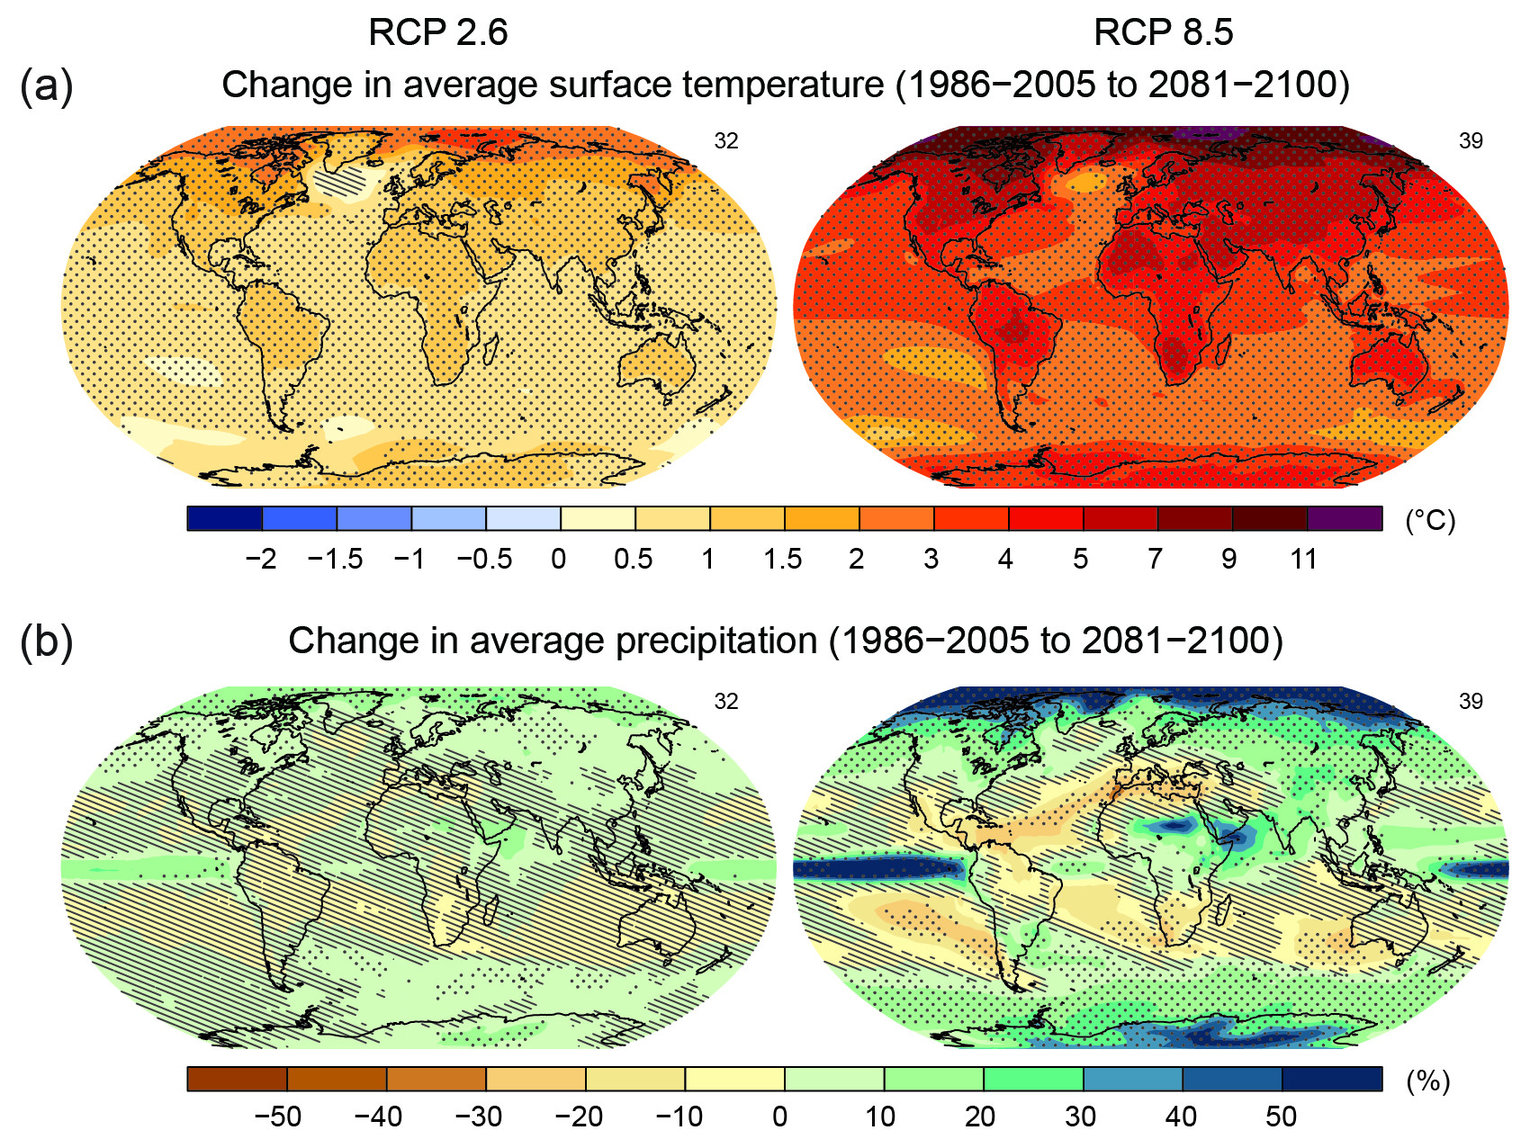
\includegraphics[width=\textwidth]{chap1/ipcc2013_T_rain_WGI_AR5}
\caption{Changement de température et de précipitation moyenne à l'horizon 2100 pour 2 scénarios du GIEC (RCP2.6 et RCP 8.5)}
\label{fig:ipcc2013_T_rain}
\end{figure}

Toutes ces perturbations posent notamment la question de la pérennité de la fonction puit de carbone de ces écosystèmes.

\index{tourbières|)}

\section{Flux de gaz à effet de serre et facteurs contrôlants}

\subsection{Les flux entre l'atmosphère et les tourbières}

\subsubsection{Les flux gazeux entrants}
%\subsection{Assimilation du carbone atmosphérique}

Le carbone est principalement présent dans l'atmosphère sous forme de dioxide de carbone (\coo) et de méthane (\chh).
Comparé au CO2, le CH4 est un GES qui est bien moins présent dans l'atmosphère (CHIFFRES!).
Cependant son "pouvoir de réchauffement" est bien plus important (effet radiatif CO2 x 100) (CHIFFRES !) (D'abord la vapeur d'eau, ensuite le CO2 et enfin le CH4)
Il est usuellement convenu (???? ref) que dans une tourbière le méthane représente environ \SI{5}{\percent} du bilan de C.
\textbf{Devenir du méthane atm}
Le transfert du \coo atmosphérique vers la biosphère (de l'atmosphère à la tourbe) est principalement \plop liée à la photosynthèse.
La photosynthèse est la réaction photochimique permettant l'assimilation du \coo par les végétaux chlorophylliens.
\textbf{dans le but de ?}.

\textbf{Détails ?}

Si la photosynthèse est un processus majeur d'assimilation du \coo, il existe d'autres voies métaboliques permettant la capture du \coo de l'atmosphère.\index{photosynthèse}
Ainsi les micro-organismes chemolithotrophes (\textbf{expliciter}) sont capables d'assimiler le \coo en utilisant l'énergie issue de l'oxydation de composés inorganiques.

Les voies métaboliques permettant l'assimilation du \coo sont plutôt bien connues (farquhar) et le fait que les substrats de départ de varient pas (sur ?) a permis une compréhension relativement fine du processus.
Cependant une fois assimilé par la végétation le devenir du carbone est moins direct.

%\subsection{Devenir du carbone assimilé}
%\subsubsection{libération du carbone ? Respiration}
\subsubsection{Les flux gazeux sortants}
Dans les tourbières le CO2 est produit par des sources multiples.
Ces sources sont la respiration des de la flore qu'elle soit aérienne ou souterraine et la respiration microbienne.\index{respiration}
Une autre source de CO2 est l'oxydation du CH4 lors de sa migration des zones anoxiques aux zones oxiques de la colonne de tourbe.
Enfin dans les zones anaérobie, le CO2 peut être produit par fermentation (respiration anaérobie).
La production de CO2 est donc un signal intégré sur l'ensemble de la colonne de tourbe. 
C'est cette multitude de processus qui rend l'estimation de ce flux difficile, en effet chacune des respirations n'aura pas la même sensibilité vis à vis de facteurs contrôlant.
La respiration de l'écosystème (RE) est définie comme l'ensemble des respirations de la colonne de tourbe, en incluant à la fois sa partie aérienne et sa partie souterraine. \index{respiration!de l'écosystème}
La respiration du sol (SR) est elle définie comme l'ensemble des respirations de la colonne de tourbe, en excluant la partie aérienne.\index{respiration!du sol}
La respiration du sol comprend donc principalement les respirations issues de la rhizosphère et des communautés de micro-organisme.

Les tourbières sont des écosystèmes dont la production primaire est estimée à environ \SI{500}{\gcm} \cite{francez2000}. 


La strate muscinale pouvant jouer/participer/produire jusqu'à \SI{80}{\percent} de la production primaire \cite{francez2000}.
Cette production primaire n'est pas particulière élevée \plop et c'est en fait la faible décomposition des matières organiques qui permet aux tourbières de stocker du carbone.
L'accumulation moyenne estimée dans les tourbières boréales est de \SI{30}{\gcm}. Le taux d'accumulation varie en fonction des espèces végétales présentes (\plop), le niveau d'eau (\plop), ... (??)



\subsubsection{storage ?}

Le carbone assimilé par photosynthèse, utilisé par la plante puis évacué que se soit sous forme d'exudats racinaire ou de matériels morts, de litière, va en partie se dégrader.
Continum de dégradation avec des matières organiques de plus en plus récalcitrantes avec la profondeur.

La vitesse de stockage au cours du temps ?

L'accumulation de matières organiques et donc de carbone dans les tourbières est donc fonction de la prépondérance relative de ces flux entre l'écosystème et l'atmosphère.

\subsection{Les facteurs majeurs contrôlant les flux}



Ces flux sont contrôlés par différents facteurs.
Parmi ceux qui sont le plus souvent cité figure la température, le niveau de la nappe et la végétation.
%Plus rarement, la disponibilité du substrat, la texture du sol le pH ou enc.
%L'intrication des différents facteurs rend difficile d'isoler

%La température
L'augmentation de la vitesse de réaction de nombreuses réactions biochimiques avec la température est connue depuis longtemps.
Elle a été mise en évidence par un chimiste suédois en 1889 : Svante August Arrhenius sur la base de travaux réalisés par un autre chimiste, néerlandais, Jacobus Henricus Van't Hoff.
Depuis, de nombreuses mesures de terrain confirment cette relation \plop
La photosynthèse et l'ensemble des respirations sont donc contrôlées, au moins en partie, par la température.

%L'hydrologie
Deuxième facteur contrôlant majeur : l'hydrologie.
L'eau joue un rôle indispensable à la formation et au maintient de ces écosystèmes.
Le niveau de la nappe, que le défini ici comme la distance entre la surface topographique de l'écosystème et le toit de l'aquifer/l'eau libre/la zone saturée.
Ce niveau sépare la colonne de tourbe en une zone oxique, ou il y a présence d'oxygène, et une zone anoxique dans laquelle l'oxygène est absent.
Cette différence va influer sur la production du \coo et du \chh.
La zone anoxique permet aux organismes anaérobies de se développer, notamment les Archaea\footnote{micro-organismes unicellulaires procaryotes} méthanogènes.
L'activité de ces organisme est la plus importante juste sous la surface de l'eau, là ou ils trouvent, en plus de l'anoxie, des matières organiques de qualité (faiblement décomposées).
La zone aérobie permet la respiration aérobie (\textbf{aérobie vs oxique}) des micro-organismes, des racines et de la faune.
C'est donc dans cette zone qu'est produit la majorité du \coo.
Lors de son transport de la zone anoxique vers la surface, le \chh passe par la zone oxique et y est en partie oxydé en \coo.
(organismes méthanotrophes)
Le niveau de la nappe contraint également le teneur en eau du sol et la hauteur de la frange capillaire (Laiho2006).
Ce point a son importance notamment pour la végétation.

%La végétation
La végétation est également un facteur important concernant les flux de gaz liés aux tourbières.
D'abord car elle exerce une influence directe sur les flux, avec d'un côté la photosynthèse et la respiration.
La photosynthèse est le seul processus\footnote{pas tout à fait exact, certains organismes peuvent se développer uniquement avec du \coo et un apport d'énergie suffisant} permettant le piégeage du carbone présent dans l'atmosphère.
Le potentiel de végétation pouvant être différent selon la plante considéré (Moore2002), la composition des communautés végétales influe donc la quantité de carbone potentiellement assimilable par l'écosystème.
La respiration des plantes que se soit via leurs parties aériennes ou souterraines (les racines) va permettre de libérer du \coo.
\textbf{(Estimation chiffres ?)}
La végétation fournie également via ses litières, des matières organiques fraîches pour les micro-organismes.
Mais la végétation peut également stimuler la respiration des micro-organismes présent dans la rhizosphère\footnote{zone du sol impacté par les racines} via la libération d'exsudats racinaires (Moore2002).
Enfin un effet indirect lié à l'adaptation de certaines plantes vasculaire aux conditions saturée en eau et anoxique.
En effet certaines plantes présentes dans ces milieux humides ont développées un Aerenchyme, un espace intercellulaire agrandit permettant le transport d'oxygène des parties aériennes de la plantes aux parties submergées.
Le transport peut également se faire dans l'autre sens et permettant par exemple le transport du \coo ou du \chh dans l'atmosphère.
Ce passage au travers de la plante permet également au \chh d'éviter d'être oxydé avant d'atteindre l'atmosphère.



%Les communautés végétales évoluent en parallèle de l'évolution de la tourbière (succession végétale).
%Les tourbières sont le siège d'une végétation caractéristique : Les sphaignes.
%Ces bryophytes sont la clef de voûte de ces écosystèmes d'abord parce que leur litière sont moins facilement dégradable que celle des espèces vasculaires.
%Ensuite parce qu'elle favorisent dans leur environnement local, les conditions favorable à leur développement. 
%On les appelle d'ailleurs des espèces ingénieures.
%Ces végétaux sans racines ont également une grande capacité à retenir l'eau (ce sont de véritables éponges) retenant également les nutriments. 
%Ceci favorisant un milieu pauvre en nutriment et donc défavorable aux autres espèces (vasculaires?).
%Il existe un grand nombre d'espèce de sphaignes (CHIFFRES+REF).
%Par la suite il ne sera pas fait de distinction entre les différentes espèces présentes sur les différents sites étudiés.
%Cependant dans de nombreuses tourbières on constate un envahissement par des végétaux vasculaires.
%Ces plantes, sont souvent des pins, des bouleaux et des molinie ?
%Elles ont un effet sur la production de CO2 principalement en aérant le sol, permettant à l'oxygène de migrer plus loin dans le profil, permettant à l'activité aérobie (plus efficace) d'agir sur une plus grande profondeur.
%Ces végétaux peuvent également pomper de l'eau en quantité (arbre?) ?


D'autres facteurs à évoquer ?

%La température est le premier facteur contrôlant les flux.
%Comme pour toute (la majorité ? y a-t-il des réactions chimiques non influencées par la température ?) les réactions chimique la température influe sur les vitesses de réactions. 
%Plus la température augmente plus la vitesse de réaction augmente.
%La température à donc un rôle important à jouer au niveau des flux.

\subsubsection{Facteurs contrôlant la respiration de l'écosystème}
\index{respiration!de l'écosystème!contrôle}
Updegraf2001\\
Montre, dans une expérimentation à base de mésocosme, que la respiration de l'écosystème est contrôlée presque exclusivement par la température du sol.

Cai2010\\
Mesures in-situ, sécheresse court terme, plus chaud et plus sec (1an).
Sensibilité à la température (Q10) identique l'année humide et l'année sèche.
Dans les conditions plus chaude et plus sèche Cai observe une augmentation de la Respiration (plus forte que celle de la photosynthèse)

Stratck2006 \\
Augmentation de la respiration suite à un abaissement du niveau de l'eau (8ans plus tôt).

Ballantyne2014 \\
dans une expérimentation in-situ, montre une respiration de l'écosystème plus importante quand le niveau de la nappe est bas que lorsque le niveau de la nappe est haut.
L'expérimentation se fait sur un site dont l'abaissement de la nappe est effectif depuis longtemps (80 ans plus tôt)
Même résultat que strack, donc effet présent même sur le long terme.

\subsubsection{Facteurs contrôlant la production primaire brute}
\index{production primaire brute!contrôle}
Si la diversité des réactions est moindre pour la photosynthèse, sa réponse aux variables environmentales à l'échelle de l'écosystème n'en est pas moins difficile à prédire.
Comme pour la respiration, l'augmentation de la température augmente la vitesse de réaction (Cai2010).
\plop
L'effet d'une variation du niveau de la nappe est cependant moins évidente.
La baisse du niveau de la nappe peut à la fois induire une augmentation de la PBB, notamment quand elle favorise la végétation vasculaire (Ballantyne2014).
Mais elle peut également la diminuer, lorsqu'elle induit un stress hydrique important (Strack \& Zuback 2013, Peichl 2014, Alm1999, Griffis2000, Weltzin2000)

\subsubsection{Facteurs contrôlant l'ENE}
\index{echange net de l'ecosystem@échange net de l'écosystème!contrôle}
On défini l'Échange Net de l'Écosystème (ENE) comme la différence entre la Photosynthèse Primaire Brute (PPB) et la Respiration de l'écosystème (RE).
Les facteurs contrôlants l'ENE sont donc les mêmes que ceux qui contrôlent ces 2 flux.
Cependant l'effet d'un même facteur de contrôle peut être différent vis à vis de PPB et de RE selon le contexte environnemental, que ce soit par rapport à la nature de l'effet ou son importance.
Ainsi une variation de l'ENE peut parfois est contrôlé majoritairement soit par la PPB soit par la RE soit par les deux.
Par exemple, une baisse du niveau de la nappe est souvent liée dans la littérature à une baisse de l'ENE.
Cependant certains attribuent cette baisse à une augmentation de la Respiration (Aurela2013, Ballantyne2014, Alm1999, Ise2008, Oechel1993) quand d'autres l'attribue à une diminution de la photosynthèe Sonnentag2010, Peicl2014.
Enfin certain voient un effet à la fois de l'augmentation de la respiration et de la diminution de la photosynthèse (StrackZuback2013)

À noter un article intéressant (Lund2012) dans lequel, dans un même site une baisse du niveau de la nappe 2 année différente entrainera une baisse de l'ENE dans les 2 cas, mais dans l'un des cas cette baisse est contrôlée par un augmentation de la respiration et dans l'autre cas cette baisse est contrôlée par une diminution de la photosynthèse.

Également un article de Ballantyne2014 qui lui ne note pas d'effet d'une baisse du niveau de la nappe sur l'ENE car l'augmentation de la respiration est compensée par une augmentation de la photosynthèse.

\subsubsection{Facteurs contrôlant les flux de méthane}

Le niveau de la nappe et la température semblent être les facteurs prépondérant du contrôle des flux de méthane
%\subsubsection{L'hydrologie dans les tourbières et l'effet sur les flux}

%\subsubsection{La végétation dans les tourbières et l'effet sur les flux}


La prépondérance relative des ces différents flux, contrôlée par les conditions environnementale, va donc impacter le fonctionnement des tourbières. 
Soit elles stockent du carbone, en accumulant des matières organiques, et donc fonctionnent comme des puits ou soit elle relâchent du carbone et fonctionnent comme des sources.


L'étude individuelle de tel ou tel flux avec tel ou tel facteur contrôlant est nécessaire afin de comprendre ce qu'il se passe au niveau des processus.
Il est tout aussi nécessaire d'arriver à intégrer l'ensemble de la complexité naturelle.
C'est l'intérêt d'établir des bilans de carbone.

\subsection{Bilans de carbone}

Le calcul d'un bilan de carbone à l'échelle d'un écosystème permet de déterminer si l'équilibre (où le déséquilibre) des flux tend à stocker du carbone, le système fonctionnant alors comme un puits, ou à libérer du carbone, le système fonctionnant alors comme une source.
Il existe différentes façon de réaliser le bilan de carbone d'une tourbière que l'on peut séparer en deux approches principales.
La première approche consiste à utiliser l'archive tourbeuse pour estimer des vitesses d'accumulation de la tourbe.
Cette méthode permet d'étudier la fonction puits sur des temps long (derniers millénaires) et de lier d'éventuels changements dans les vitesses d'accumulation à des facteurs environnementaux.
La seconde approche se base d'avantage sur des mesures actuelles des différents flux afin d'étudier, sur des temps forcément plus court, l'évolution de la prépondérance puits/source d'un écosystème.
Les deux approches sont donc complémentaires.

\subsubsection{passé}
long-term apparent rate of carbon accumulation (LORCA) 
datations + dry bulk density + carbon content
(Tableau~\ref{table:lorca})

\begin{table}
\centering
\caption{Vitesse apparente d'accumulation du carbon à long terme en \si{\gcms}}
\label{table:lorca}
\begin{tabular}{llp{7cm}}\toprule
min -- max & moyenne & référence \\ \midrule
20 -- 140  & ? & Mitra2005 \\ %Xing
? & 18.6 &  Yu2009\\  %Xing
 & 17.2 & Gorham2012 \\  %Xing
 & 20 & Jones2010\\  %Xing
 & 16.2 & Borren2004\\  %Xing
 & 18.5 & Packalen2014\\ %Xing
 & 19.4 & Vitt2000\\ %Roulet2007
 & 19 & Turunen2004\\ %Roulet2007 (ombrotrophic bog)
5.74 -- 129.31 & 33.66 & Xing2015\\
\bottomrule
%CAR : 18.6 turunen2002 in Roulet2007
\end{tabular}
\end{table}
\textbf{tableau LORCA ajouter colonne contexte (exple: 7 tourbières ombrotrophes)}

\subsubsection{présent}
Dans cette approche on estime les flux actuels de carbone entrant et sortant de l'écosystème afin de déterminer un bilan.
Un certain nombre de flux de carbone sont présent au sein des écosystèmes terrestre (équation~\eqref{bdc})

\begin{equation}
BCNE=\frac{dC}{dt}=\overbrace{PPB - Re}^{ENE}  - F_{COD} - F_{COP} - F_{CH_{4}} \textcolor{gray}{- F_{CID} - F_{COV} - F_{CO}}
\label{bdc}
\end{equation}

\begin{itemize}
\item ENE : Échange Net de l'Écosystème
\item PPB : Production Primaire Brute
\item Re : Respiration de l'Écosystème
\vspace*{.2cm}
\item F$_{COP}$ : Flux de Carbone Organique Dissous
\item F$_{COP}$ : Flux de Carbone Organique Particulaire
\item F$_{CH_{4}}$ : Flux de Méthane
\vspace*{.2cm}
\item \textcolor{gray}{F$_{CID}$ : Flux de Carbone Inorganique Dissous}
\item \textcolor{gray}{F$_{COV}$ : Flux de Composés Organique Volatils}
\item \textcolor{gray}{F$_{CO}$ : Flux de Monoxyde de Carbone}
\end{itemize}

Les bilans les plus complets réalisées sur les tourbières comprennent la partie gazeuse, dissoute...

Dans les tourbières, les flux de \coo sont généralement les plus importants \plop, puis les flux de \chh et/ou de COD et enfin les flux de COP.

Pour estimer ces flux différentes techniques existent, notamment l'eddy covariance et les méthodes de chambre pour les flux de gaz.

D'autres méthodes, moins souvent utilisées, existent comme l'utilisation du ratio C:N (Kirk2015)


%\section{Objectifs du travail}